\section{Results}


% In order to evaluate and compare federated learnign models 
% Specificity  and  sensitivity  are  the  abilities  of  a  model  that how correctly the model identifies a subject with disease and without a disease. 
% In our case, it is critical to detect a COVID-19 patient as missing a COVID-19 patient can have disastrous consequences.   

% A medical diagnosis based system needs to have high sensitiv- ity and recall. 
Here, the result for the setting with 10 participating clients and a maximum of 10 rounds is presented. The results are average performance among clients for all the federated rounds. Table \ref{best_performance} shows the results.
% \quickthings{Why comparison of FedAVG and CWT?}\maybelater{I removed the sentence}
% The average score in each state could be a way to reach them—the average scores in F1, FedSGD, CWT, and SWT. 
% The FedSGD models have been used are
% The results for CDS are also included as a benchmark ground truth.

% \quickthings{Put CDS at the top, keep same order as in the materials and methods. Consistency!}
% \maybelater{Fixed!}

\begin{table}[h!]
\centering
\setlength{\tabcolsep}{5.5pt}
\renewcommand\arraystretch{1.12}
\caption{ \small Comparison of FL algorithms on classification of COVID-19 data for 10 clients, averaged performance in all the 10 rounds.}
\begin{tabular}{| *{5}{c|} }
\hline
Method & Accuracy & Recall & Precision & F1 score
\\
  \hline
  

CDS
 &87.75\%&89.57\% &87.93\% & 87.19\%  
\\   \hline  
FedAVG
 & 66.72\% &70.02\% &43.80\% & 51.7\%\\ 
 \hline  
FedSGD
 &65.17\% &68.24\%&43.86\%& 47.75\%  
 
 \\
 \hline  
CWT
 &87.75\%&89.00\%& 88.67\%&87.52\%\\
 
   \hline
 

SWT
 & 64.60\% &74.33\% & 65.55\% &59.66\% \\
    
\hline 
STWT
 & 84.21\% &84.09\%&83.33\% & 81.71\%  \\



\hline
\end{tabular}
\label{best_performance} 
\end{table}


\textbf{Assesing the impact of training rounds} To evaluate the effect of number of rounds, models with 3, 5, 10 and 15 rounds were tested. The test results are shown for both centralized and FL  algorithms. Table \ref{number_of_rounds} shows the results of our experiment. The increasing number of rounds correlates with higher accuracy of the global model.
% \quickthings{Same with table III, put at the top.}

% \maybelater{done}

% \begin{table}[h!]
% \centering
% \setlength{\tabcolsep}{5.5pt}
% \renewcommand\arraystretch{1.12}
% \caption{ \small Effect number of rounds on models' accuracy}
% \begin{tabular}{| *{5}{c|} }
% \hline
% Method & 3 rounds & 5 rounds & 10 rounds & 15 rounds 
% \\   \hline  
% FedAVG
%  & 66.28\% &77.24\% & 86.63\% & 94.03\%\\

%  \hline
%  FedSGD
%  &  53.77\% & 70.55\% &90.04\% & 92.75\%\\
% \hline  
% % SWT
% %  &  85.34\% & 97.24\% &93.63\% & 98.74\%\\
% % \hline  
% CWT
%  &  96.02\% & \textbf{98.44\%} &\textbf{99.29\%} & 99.86\%\\

% % \hline  
% % CDS
% %  to be completed!


% \hline  
% STWT
%  &  \textbf{96.59\%} & 97.72\% &99.57\% & \textbf{100.00\%}\\

 
%  \hline
% CDS
%  &92.03\% &88.34\% & 98.01\% & 100.00\% \\
%  \hline
% \end{tabular}
% \label{number_of_rounds} 
% \end{table}


\begin{table}[h!]
\centering
\setlength{\tabcolsep}{3.5pt}
\renewcommand\arraystretch{1.12}
\caption{ \small Effect number of rounds on accuracy of FL algorithms for 10 clients, 20 internal epochs.}
\begin{tabular}{| *{5}{c|} }

% \begin{tabular}{| {c|}{c|}{c|}{c|}{c|}{c|}{c|}{c|}{c|} |}
\hline
% Method & \multicolumn{2}{c}{3 rounds} & \multicolumn{2}{c}{5 rounds} &\multicolumn{2}{c}{10 rounds} &\multicolumn{2}{c}{15 rounds} 

Method & 3 rounds & 5 rounds & 10 rounds & 15 rounds
%  & M &SD & M &SD& M &SD& M &SD 
\\
 \hline
CDS
 &85.06\% &81.56\% & 91.06\% & 91.04\% 
\\
\hline
FedAVG
 & 56.05\%  &63.78\%&69.64\%&70.73\% \\

 \hline
 FedSGD
 &  50.88\% & 55.9\% &75.59\% & 76.94\%\\
% \hline  
% SWT
%  &  85.34\% & 97.24\% &93.63\% & 98.74\%\\
\hline  
CWT
 &  80.77\% & \textbf{89.78\%} &\textbf{91.27\%}& \textbf{93.56\%}\\

% \hline  
% CDS
%  to be comp,';leted!


\hline  
STWT
 &  \textbf{90.73\%} & 83.97\% &89.44\% & 93.01\%\\

 
  \hline

\end{tabular}
\label{number_of_rounds} 
\end{table}
\quickthings{Shouldn't this column have the same results as table II for accuracy?}

\peter{Table III and Table II do not represent the same thing. Table II is average performance in all 10 rounds, is to give an overall impression of accuracy, and table III is the final result in the end of the 5th, 10th , 15th rounds.  Added  to the table caption.
}
% \maybelater{The results are for max, maybe you want to add average results later?}
% \maybelater{Having the same thing (acc) for other metrics such as F1, prevciison recall etc}

\textbf{Assessing the influence of client participation}
To evaluate the number of clients on the FL network, we examined scenarios with 3,5, and 8 participating clients. We trained each of the clients in 20 internal epochs. The number of Federated rounds for all the algorithms (except SWT) was 10.
The average test results are shown in the Figure \ref{fig:data distribution}. \quickthings{Why not a column for 10 clients here?}
\maybelater{ 10 clients are shown in table three , third column. Added 10 clients here as well}

% \begin{table}[h!]
% \centering
% \setlength{\tabcolsep}{7pt}
% \renewcommand\arraystretch{1.22}
% \caption{ \small Effect number of clients on accuracy of FL algorithms, 10 rounds, 20 internal epochs.}
% \begin{tabular}{| *{9}{c|} }
% \hline
% Method & 3 clients & 5 clients & 8 clients 
% \\   \hline  
% FedAVG
%  & 79.52\% &70.73\% & 63.98\% \\

% \hline  
% FedSGD
%  & 78.02\% &75.59\% &69.76\%  \\
% \hline  
% CWT
%  &  89.90\% & \textbf{91.27\%} &\textbf{88.98\%} \\
%  \hline
% STWT
%  &  \textbf{90.93\%} & 89.44\% &84.57\% \\
%  \hline  
% SWT
%  & 55.80\% &69.19\% & 68.81\%\\




% \hline  
% CDS
%  to be completed!

% \hline  

% \end{tabular}
% \label{effect_num_clients} 
% \end{table}


\begin{figure}[h!]
 \centering
 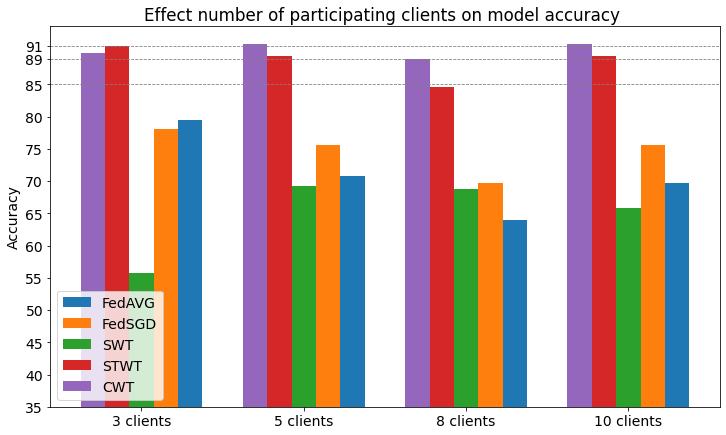
\includegraphics[width=0.7\textwidth]{download.png}
 \caption{Accuracy of FL algorithms with differrent number of clients. }
 \label{fig:data distribution}
\end{figure}


% \maybelater{Maybe taking MAX is better instead of latest epoch?}

 
\begin{figure}[h!]
 \centering
 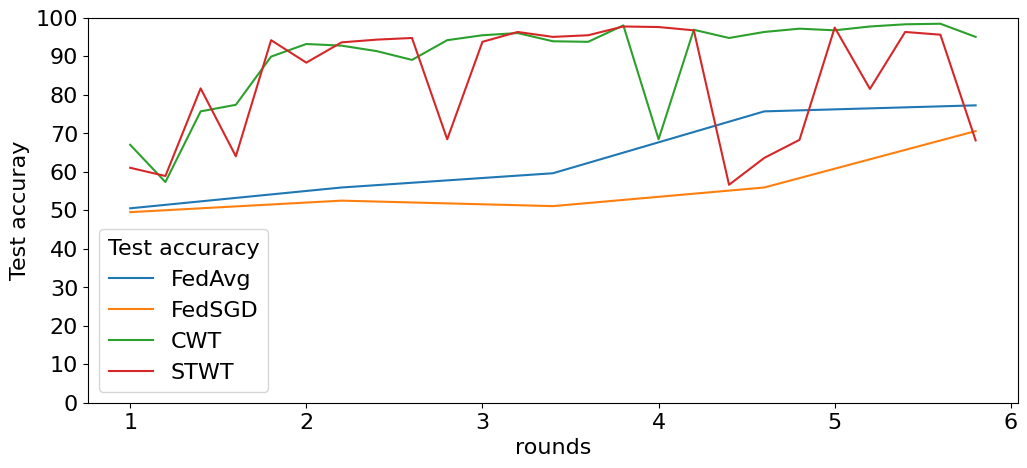
\includegraphics[width=0.7\textwidth]{cyclic.png}
 \caption{Test accuracy as a function of passing rounds}
 \label{seq-vs-noseq}
\end{figure}
% \maybelater{Best accuracy vs Average accuracy for showing that SWTW works bad in average but well in best accuracy}
% \abs{Adding a graph showing arrows for gradient updates}
% \maybelater{Maybe adding 10 clients?}
% \maybelater{8 ta client, 4 FL rounds
% 20 each client for CWT plot . and also 8 ta client, 4 FL round 20 each client for FedSGD and FedAVG}
% \subsection{Other graphs}

\begin{table}[h!]
\label{computation time}
\centering
\setlength{\tabcolsep}{7pt}
\renewcommand\arraystretch{1.22}
\caption{ \small Computation time (seconds) for FL algorithms for standardized setting}
\begin{tabular}{| *{9}{c|} }
\hline
Method & 3 clients & 5 clients & 8 clients  & 10 clients
\\   \hline  
FedAVG
 & 8934 sec&8975 sec  & 9002 sec & 9030 sec\\

\hline  
FedSGD
 & 8810 sec &8853 sec& 9013 sec & 9052 sec \\
\hline  
CWT
 &  5119 sec& 5450 sec&5383 sec & 5556 sec\\
 \hline
STWT &
2805 sec&  5243 sec& 6101 sec & 6129 sec\\
 \hline  
SWT
 & \textbf{543 sec} &\textbf{547 sec} & \textbf{589 sec } & \textbf{618 sec}\\



% \hline  
% CDS
%  to be completed!

\hline  

\end{tabular}
\label{computation_time} 
\end{table}


Communication can also be a bottleneck in this setting. In methods like federated averaging, the lower bounds for total communicated data are proportional to $\sim$
${2NT}$
where the total rounds are represented by T and the count of involved clients is denoted by N. In CWT, this lower bound is  $\sim$ ${NT}$. In our setting, we use a ResNet 101 model. We calculated the overall transferred data for the different number of rounds. As expected, the experiments show that when clients are selected randomly, the communication time tends to be shorter compared to scenarios involving participation from all clients. Moreover, our analysis of computational costs indicates that models that do not rely on sequential processing generally demand higher computational resources compared to their sequential counterparts. The detailed results for computational and communication evaluations can be found in Table \ref{computation_time} and Table \ref{transferredData}, respectively.
\quickthings{Again, why only this comparison is relevant enough to put into the text?}
\maybelater{Here fedavg, and fedsgd are the same family, (non sequential), and CWT are the other family (sequential)., Changed the phrasing from CWT/FedAVG to seq/non-seq, hope it's okay this time.}

\begin{table}[h!]
\centering
\label{Transferred data}
\setlength{\tabcolsep}{5.5pt}
\renewcommand\arraystretch{1.12}
\caption{ \small Comparison of total transferred data in a normalized setting (GB)}
\begin{tabular}{| *{5}{c|} }
\hline
Method & 3 rounds & 5 rounds & 10 rounds & 15 rounds 
\\   \hline  
FedAVG
 & 1.371 &2.286 & 4.571 & 6.857\\

 \hline
 FedSGD
 &  0.823 & 1.371 &2.743 & 4.114\\
\hline  
% SWT
%  &  85.34\% & 97.24\% &93.63\% & 98.74\%\\
% \hline  
CWT
 &  0.686 & 1.143 &2.286 & 3.428\\

% \hline  
% CDS
%  to be completed!


\hline  
STWT &
  0.411 & 0.686 &1.371 & 2.057\\

 

 \hline
\end{tabular}
\label{transferredData} 
\end{table}





% \maybelater{Momkene computational complexity ro beshe ba order nevesht? peida kon settingesh ro}
% \maybelater{Graphs showing results}
% \maybelater{Comparison of FL models}
% \maybelater{Loss/round}
% \abs{definition of precision and recall}


\label{sec:results}


